\chapter{Introducción}

\section{Contexto y motivación}

Las simulaciones Monte Carlo son la herramienta estándar cuando la complejidad geométrica o la marcada anisotropía angular del flujo neutrónico dificultan la aplicación de métodos determinísticos. Sin embargo, cuando las partículas atraviesan blindajes o regiones altamente absorbentes, la estadística disponible en la zona de interés se reduce considerablemente, lo que incrementa la incertidumbre en magnitudes físicas clave como el flujo escalar o la dosis equivalente ambiental, e incluso puede imposibilitar su cálculo debido a nula estadística. 

En este trabajo abordaremos la temática de la obtención de resultados a la salida de canales de extracción de neutrones en reactores de investigación tipo pileta. En estos sistemas, los neutrones generados en el núcleo deben atravesar el agua de la pileta antes de alcanzar la entrada del canal de extracción. Durante una simulación desde el núcleo, la mayoría de los neutrones permanecen dentro del mismo y aquellos que logran salir al agua son en gran medida absorbidos a medida que penetran en esta. En consecuencia, son escasos los neutrones que finalmente alcanzan la entrada del canal, haciendo que resulte computacionalmente costoso obtener estadística suficiente a la salida del canal, en el ambiente circundante o en dispositivos experimentales.

En la Figura \ref{fig:nucleo2} se presenta un esquema ilustrativo del núcleo de un reactor de investigación tipo pileta con un canal de extracción de neutrones. Este esquema consta de un núcleo central rodeado por agua y rodeado externamente por un blindaje biológico. El canal de extracción permite obtener un haz de neutrones destinado a usos posteriores en investigaciones experimentales. Además, se muestra esquemáticamente mediante un gradiente de color las regiones con mayor estadística neutrónica y cómo esta disminuye drásticamente al avanzar por el agua y el blindaje. Este esquema ejemplifica una simulación típica de núcleo, ilustrando claramente las dificultades que se tienen para obtener estadística lejos del núcleo.

\begin{figure}[H]
    \centering
    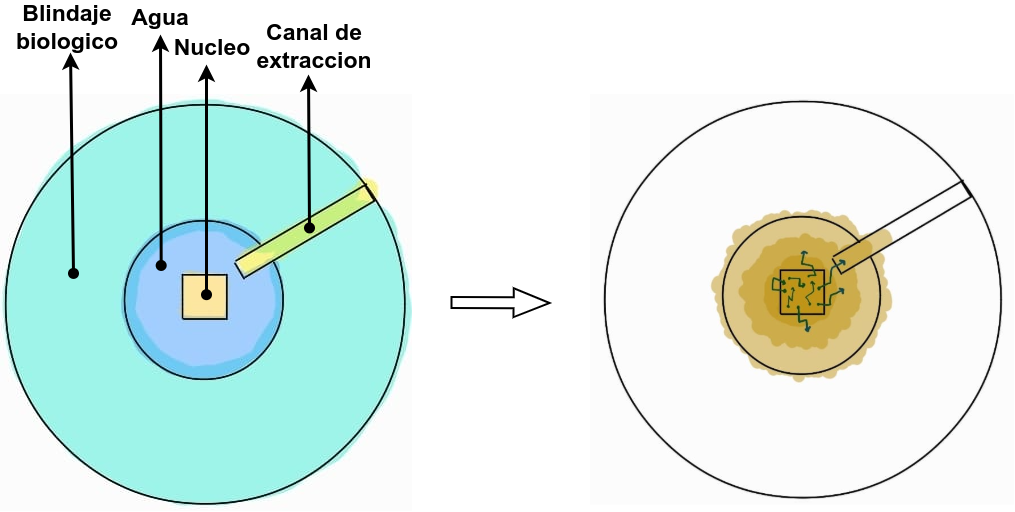
\includegraphics[width=0.8\textwidth]{nucleo2.png}
    \caption{Representación esquemática del núcleo de un reactor tipo pileta con canal de extracción. Se observa el núcleo central, rodeado por agua y blindaje biológico, así como un canal de extracción de neutrones. El gradiente de color indica cualitativamente la distribución de la población neutrónica típica en simulaciones Monte Carlo desde el núcleo.}
    \label{fig:nucleo2}
\end{figure}

Para mitigar esta problemática, se suelen emplear técnicas de reducción de varianza tales como:
\begin{itemize}
    \item \textbf{Separación geométrica del problema}: consiste en dividir la simulación en regiones contiguas, separando la fuente original de la región de interés mediante una superficie de interfaz. En dicha superficie se registran las variables del espacio de fases y el peso estadístico de las partículas que la atraviesan, con el objetivo de construir una nueva fuente de partículas estadísticamente equivalente. Esta nueva fuente permite reiniciar la simulación a partir de dicha superficie, concentrando los recursos computacionales exclusivamente en la región de interés. Existen diversos métodos para modelar este tipo de fuentes distribucionales a partir del archivo de partículas registrado, tales como el ajuste de funciones unidimensionales o multidimensionales, el método de \textit{smearing} utilizado en \textit{McStas} \cite{McStas2020Manual}, la estimación por densidad de kernels (\textit{Kernel Density Estimation}, KDE) adaptativa \cite{Schmidt2022KDSourcePaper}, o el uso de histogramas multidimensionales \cite{Fairhurst2017Hist}.
    
    \item \textbf{Absorción implícita}: en lugar de eliminar partículas cuando son absorbidas, se les reduce su peso estadístico de acuerdo a la probabilidad de absorción, permitiendo que las partículas sobrevivan y continúen su historia.
    
    \item \textbf{Ruleta rusa}: se aplica para eliminar partículas con bajo peso estadístico, preservando el valor esperado del cálculo. Esta técnica se utiliza típicamente en conjunto con la absorción implícita, ya que sin ella todas las partículas mantienen peso unitario y la aplicación de ruleta rusa no sería necesaria. Cada partícula con peso inferior a un umbral predefinido tiene una cierta probabilidad de ser eliminada; si sobrevive, su peso es incrementado.

    \item \textbf{Ventanas de peso}: esta técnica define un rango aceptable de pesos estadísticos para las partículas en cada región del dominio. Aquellas con peso muy alto son divididas (\emph{splitting}) y las de peso muy bajo se someten a ruleta rusa para controlar la varianza espacialmente.
\end{itemize}

El método desarrollado en este trabajo se basa en la separación geométrica del problema en dos regiones: una que contiene el núcleo del reactor, y otra que abarca exclusivamente la región de interés. Esta técnica se implementa mediante la división del modelo simulado en dos regiones, delimitadas por superficies de acople ubicadas estratégicamente dentro de la geometría. En una primera etapa, se realiza una simulación completa del núcleo hasta una superficie intermedia, donde se registran en una lista las propiedades de las partículas que la atraviesan, incluyendo su energía E, posición \textbf{r}, dirección $\mathbf{\Omega}$, peso estadístico, y tipo de partícula (por ejemplo, neutrón o fotón). A partir de esta lista de partículas, se estima la distribución multidimensional en el espacio de fases utilizando histogramas multidimensionales. Esta estructura permite segmentar el conjunto original de datos mediante histogramas de baja resolución, llamados histogramas macro, que separan el espacio de fases en regiones donde las correlaciones entre variables se mantienen aproximadamente constantes. Sobre cada una de estas regiones, se construyen histogramas de mayor resolución —los histogramas micro— que aproximan la distribución de cada variable con mayor detalle. De este modo, se preservan tanto la forma general de la distribución como las correlaciones entre las variables registradas. A partir de esta estimación, es posible generar nuevas partículas que pertenezcan estadísticamente al mismo espacio de fases que la muestra original, obteniendo así una fuente sintética denominada fuente distribucional. Esta metodología se desarrolla en profundidad en el Capítulo \ref{cap:metodo_histogramas}, donde se describe el procedimiento implementado para su construcción.

En la Figura~\ref{fig:nucleo4} se ejemplifica el proceso desarrollado para una simulación del núcleo de un reactor de investigación tipo pileta. Inicialmente, se realiza una simulación completa desde el núcleo, obteniendo una estadística adecuada en sus alrededores, la cual se reduce considerablemente a medida que los neutrones penetran en el agua circundante. Este fenómeno se visualiza mediante un gradiente de colores. En esta simulación se define una superficie de registro en la entrada de un canal de extracción, y las partículas que la atraviesan se registran en un archivo. A partir de dicho archivo, se construye una fuente distribucional mediante la metodología desarrollada en este trabajo. Esta fuente permite simular únicamente el canal, concentrando la estadística en esa región sin necesidad de simular desde el núcleo. En esta segunda simulación, la región previa a la superficie de interfaz se reemplaza completamente por vacío, dejando en el modelo únicamente la región de interés. Esto se logra definiendo una condición de vacío en la superficie de interfaz. Cabe destacar que, si bien podría existir la posibilidad de que alguna partícula inicialmente dirigida hacia la región de la fuente reingrese a la región de interés por retrodispersión, dicho fenómeno ya está estadísticamente incorporado en la lista original de partículas registrada en la primera simulación.

En resumen, el procedimiento consta de tres etapas fundamentales:

\begin{itemize}
    \item \textbf{Detección}: Registro de las variables del espacio de fases y del peso estadístico de cada partícula que atraviesa una superficie intermedia de desacople. El resultado de este proceso es un archivo de partículas que contiene la información necesaria para caracterizar la distribución de la fuente sobre dicha superficie.

    \item \textbf{Estimación}: Procesamiento del archivo de partículas mediante la metodología propuesta en este trabajo, basada en histogramas multidimensionales. Este procedimiento permite aproximar la distribución en el espacio de fases, preservando las correlaciones entre variables, y genera como resultado una fuente distribucional.

    \item \textbf{Producción}: Utilización de la fuente distribucional estimada para generar nuevas partículas que pertenezcan al espacio de fases del archivo de partículas original. Estas partículas son empleadas en simulaciones posteriores, permitiendo modelar la región de interés de forma desacoplada de la fuente original.
\end{itemize}

\begin{figure}[H]
    \centering
    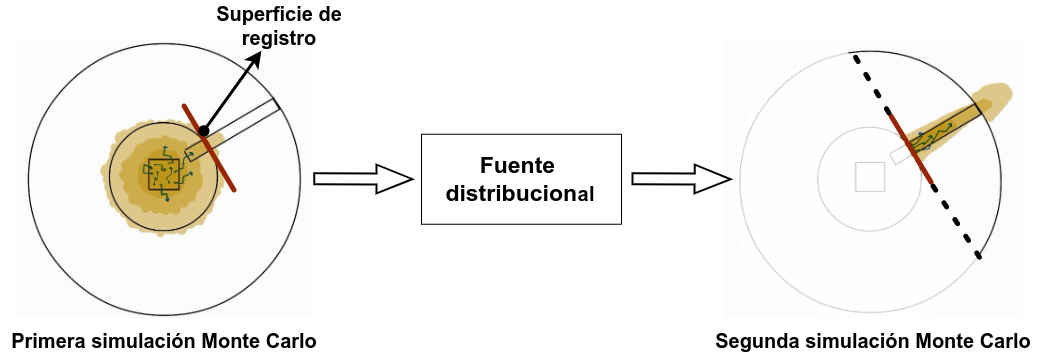
\includegraphics[width=\textwidth]{nucleo4.png}
    \caption{Esquema ilustrativo del proceso de desacople geométrico en simulaciones Monte Carlo para un reactor de investigación tipo pileta. En la primera etapa se registra un archivo de partículas en la entrada del canal de extracción, el cual es posteriormente utilizado para generar una fuente distribucional que permite simular eficientemente el canal de forma independiente. El gradiente de colores representa la disminución de la población neutrónica.}
    \label{fig:nucleo4}
\end{figure}

El archivo original de partículas contiene inevitablemente regiones del espacio de fases con baja estadística o sin eventos registrados, producto de su carácter finito. Si se reutiliza directamente como fuente en una simulación posterior —por ejemplo, simulando varias veces las mismas partículas registradas— se corre el riesgo de reproducir el mismo ruido estadístico, afectando la calidad de los resultados.

% Para mitigar este problema, se emplea un procedimiento de estimación basado en histogramas multidimensionales que permite densificar el espacio de fases. En este enfoque, se utilizan histogramas para aproximar la distribución de variables, bajo el supuesto de que la probabilidad es constante dentro de cada bin. Esto habilita la generación de nuevas partículas en regiones que no estaban presentes explícitamente en el archivo original, completando así los vacíos estadísticos y asegurando una cobertura más uniforme del espacio de fases.

\section{Trabajos relacionados}

Los trabajos previos realizados en el Departamento de Física de Reactores y Radiaciones (DeFRRa) del Centro Atómico Bariloche (CAB) \cite{DeptoReactoresNeutronesCAB2025} abordaron el modelado de fuentes distribucionales mediante el uso de histogramas multidimensionales \cite{Fairhurst2017Hist, Ayala2019Hist, Abbate2020Hist}. Esta estrategia permitió capturar correlaciones entre energía, posición y dirección en geometrías planas rectangulares, siendo aplicada satisfactoriamente en estudios vinculados al reactor RA‑10.

En continuidad con dichos desarrollos, la herramienta \texttt{KDSource} — desarrollada en conjunto por la Comisión Nacional de Energía Atómica (CNEA) \cite{CNEA2025} y por el Instituto Balseiro (IB) \cite{IB2025}— introdujo técnicas más avanzadas basadas en \textit{Kernel Density Estimation} (\textit{KDE}), en forma multivariable y adaptativa \cite{Abbate2021KDSource, Schmidt2022KDSourcePaper, Fox2022KDE, Gimenez2024KDSourceOpenMC}. \texttt{KDSource} permite ajustar automáticamente distribuciones continuas a partir de archivos de partículas previamente obtenidos y, a partir de ellas generar fuentes distribucionales, preservando las correlaciones del espacio de fases. Estas fuentes pueden ser utilizadas directamente en simulaciones Monte Carlo mediante el código \texttt{OpenMC} \cite{OpenMC2024}.

No obstante, el enfoque basado en \textit{KDE} presenta una limitación: su carácter inherentemente suavizante puede dificultar la representación precisa de discontinuidades abruptas en el espacio de fases. En particular, el método puede fallar al capturar regiones donde las distribuciones presentan derivadas segundas muy marcadas o donde ocurren cambios bruscos, como bordes definidos por condiciones geométricas o materiales. En estos casos, la suavizacion de las distribuciones multivariables puede degradar la calidad de la fuente generada, especialmente cuando se busca preservar estructuras finas o anisotropías marcadas.

El presente trabajo extiende estas líneas incorporando los enfoques basados en histogramas multidimensionales dentro del entorno ya establecido de \texttt{KDSource}, proponiendo además un método de discretización adaptativa que automatiza la definición de las grillas de los histogramas macro y micro. A diferencia de los trabajos anteriores, este nuevo enfoque permite segmentaciones variables para diferentes subconjuntos del espacio de fases. Por ejemplo, el método puede asignar una discretización angular más refinada para neutrones rápidos, donde suelen prevalecer anisotropías asociadas a haces colimados, y una discretización más homogénea para neutrones térmicos, cuya distribución tiende a ser más isotrópica. De esta forma, se logra preservar las correlaciones relevantes sin imponer una malla uniforme en todo el dominio, mejorando la capacidad de representación del método.

\section{Aportes específicos de este trabajo}

Este trabajo busca profundizar el desarrollo de \texttt{KDSource} mediante la incorporación de histogramas multidimensionales como una alternativa -o complemento- a la metodología \textit{KDE} existente. Las contribuciones específicas son:

\begin{itemize}
    \item Implementación de histogramas multidimensionales en \texttt{KDSource}, capaces de:
    \begin{itemize}
        \item preservar las correlaciones entre variables ($\mathbf{E}$–$\mathbf{r}$–$\boldsymbol{\Omega}$) para fuentes definidas sobre un plano;
        \item representar adecuadamente discontinuidades o picos en todas las variables;
        \item implementar un método de selección automática y adaptativa de bordes para los histogramas, tanto a nivel macro como micro, optimizado según la estadística disponible en cada subgrupo del espacio de fases.
    \end{itemize}

    \item Integración optimizada del flujo de trabajo en \texttt{OpenMC} mediante:
    \begin{itemize}
        \item generación \emph{offline} de un archivo intermedio en formato \texttt{XML} conteniendo la fuente distribucional, que incluye la información de los histogramas multidimensionales;
        \item desarrollo de un módulo en \texttt{C} que utilice eficientemente esta información para producir partículas individualmente;
        \item implementación de un remuestreo \emph{on-the-fly} integrado en \texttt{OpenMC}, minimizando la ocupación de memoria al evitar la carga y gestión de archivos extensos de partículas.
    \end{itemize}

    \item Validación  del método en casos de complejidad creciente:
    \begin{itemize}
        \item Un caso simplificado, consistente en un haz colimado ingresando en un paralelepípedo de agua atravesado por un canal de vacío, con fuentes definidas artificialmente para permitir una comparación con una simulación directa más extensa sin la aplicación del método desarrollado. 
        \item Un caso real, consistente en la propagación a través del conducto Nº5 del reactor RA‑6, utilizando un archivo de partículas proporcionado por el departamento de Física de Neutrones del CAB, que fue generado a través de una simulación del núcleo en \texttt{OpenMC}.
    \end{itemize}
\end{itemize}
